\newpage
\section{Implementacje}
\paragraph{}
Rozdział prezentuje różne podejścia do stworzenia implementacji przykładowej sceny w w technologii rozszerzonej rzeczywistości.
Jako środowisko badawcze wybrano salę - labolatorium znajdującą się w PJATK. Salę tę wybrano ponieważ znajduje się w podpiwniczeniu, co za tym idzie ilość światła dziennego jest znikoma, lecz wystarczająca do zastosowania urządzeń projekcyjnych w ciągu dnia. Dodatkowo w sali znajduje się rura ciepłownicza poprowadzona po dwóch ścianach. Umiejscowienie tego elementu pozwala go wykorzystać do stworzenia wirtualnej sceny (np. animacja fal wody w środku rury).

\begin{center}
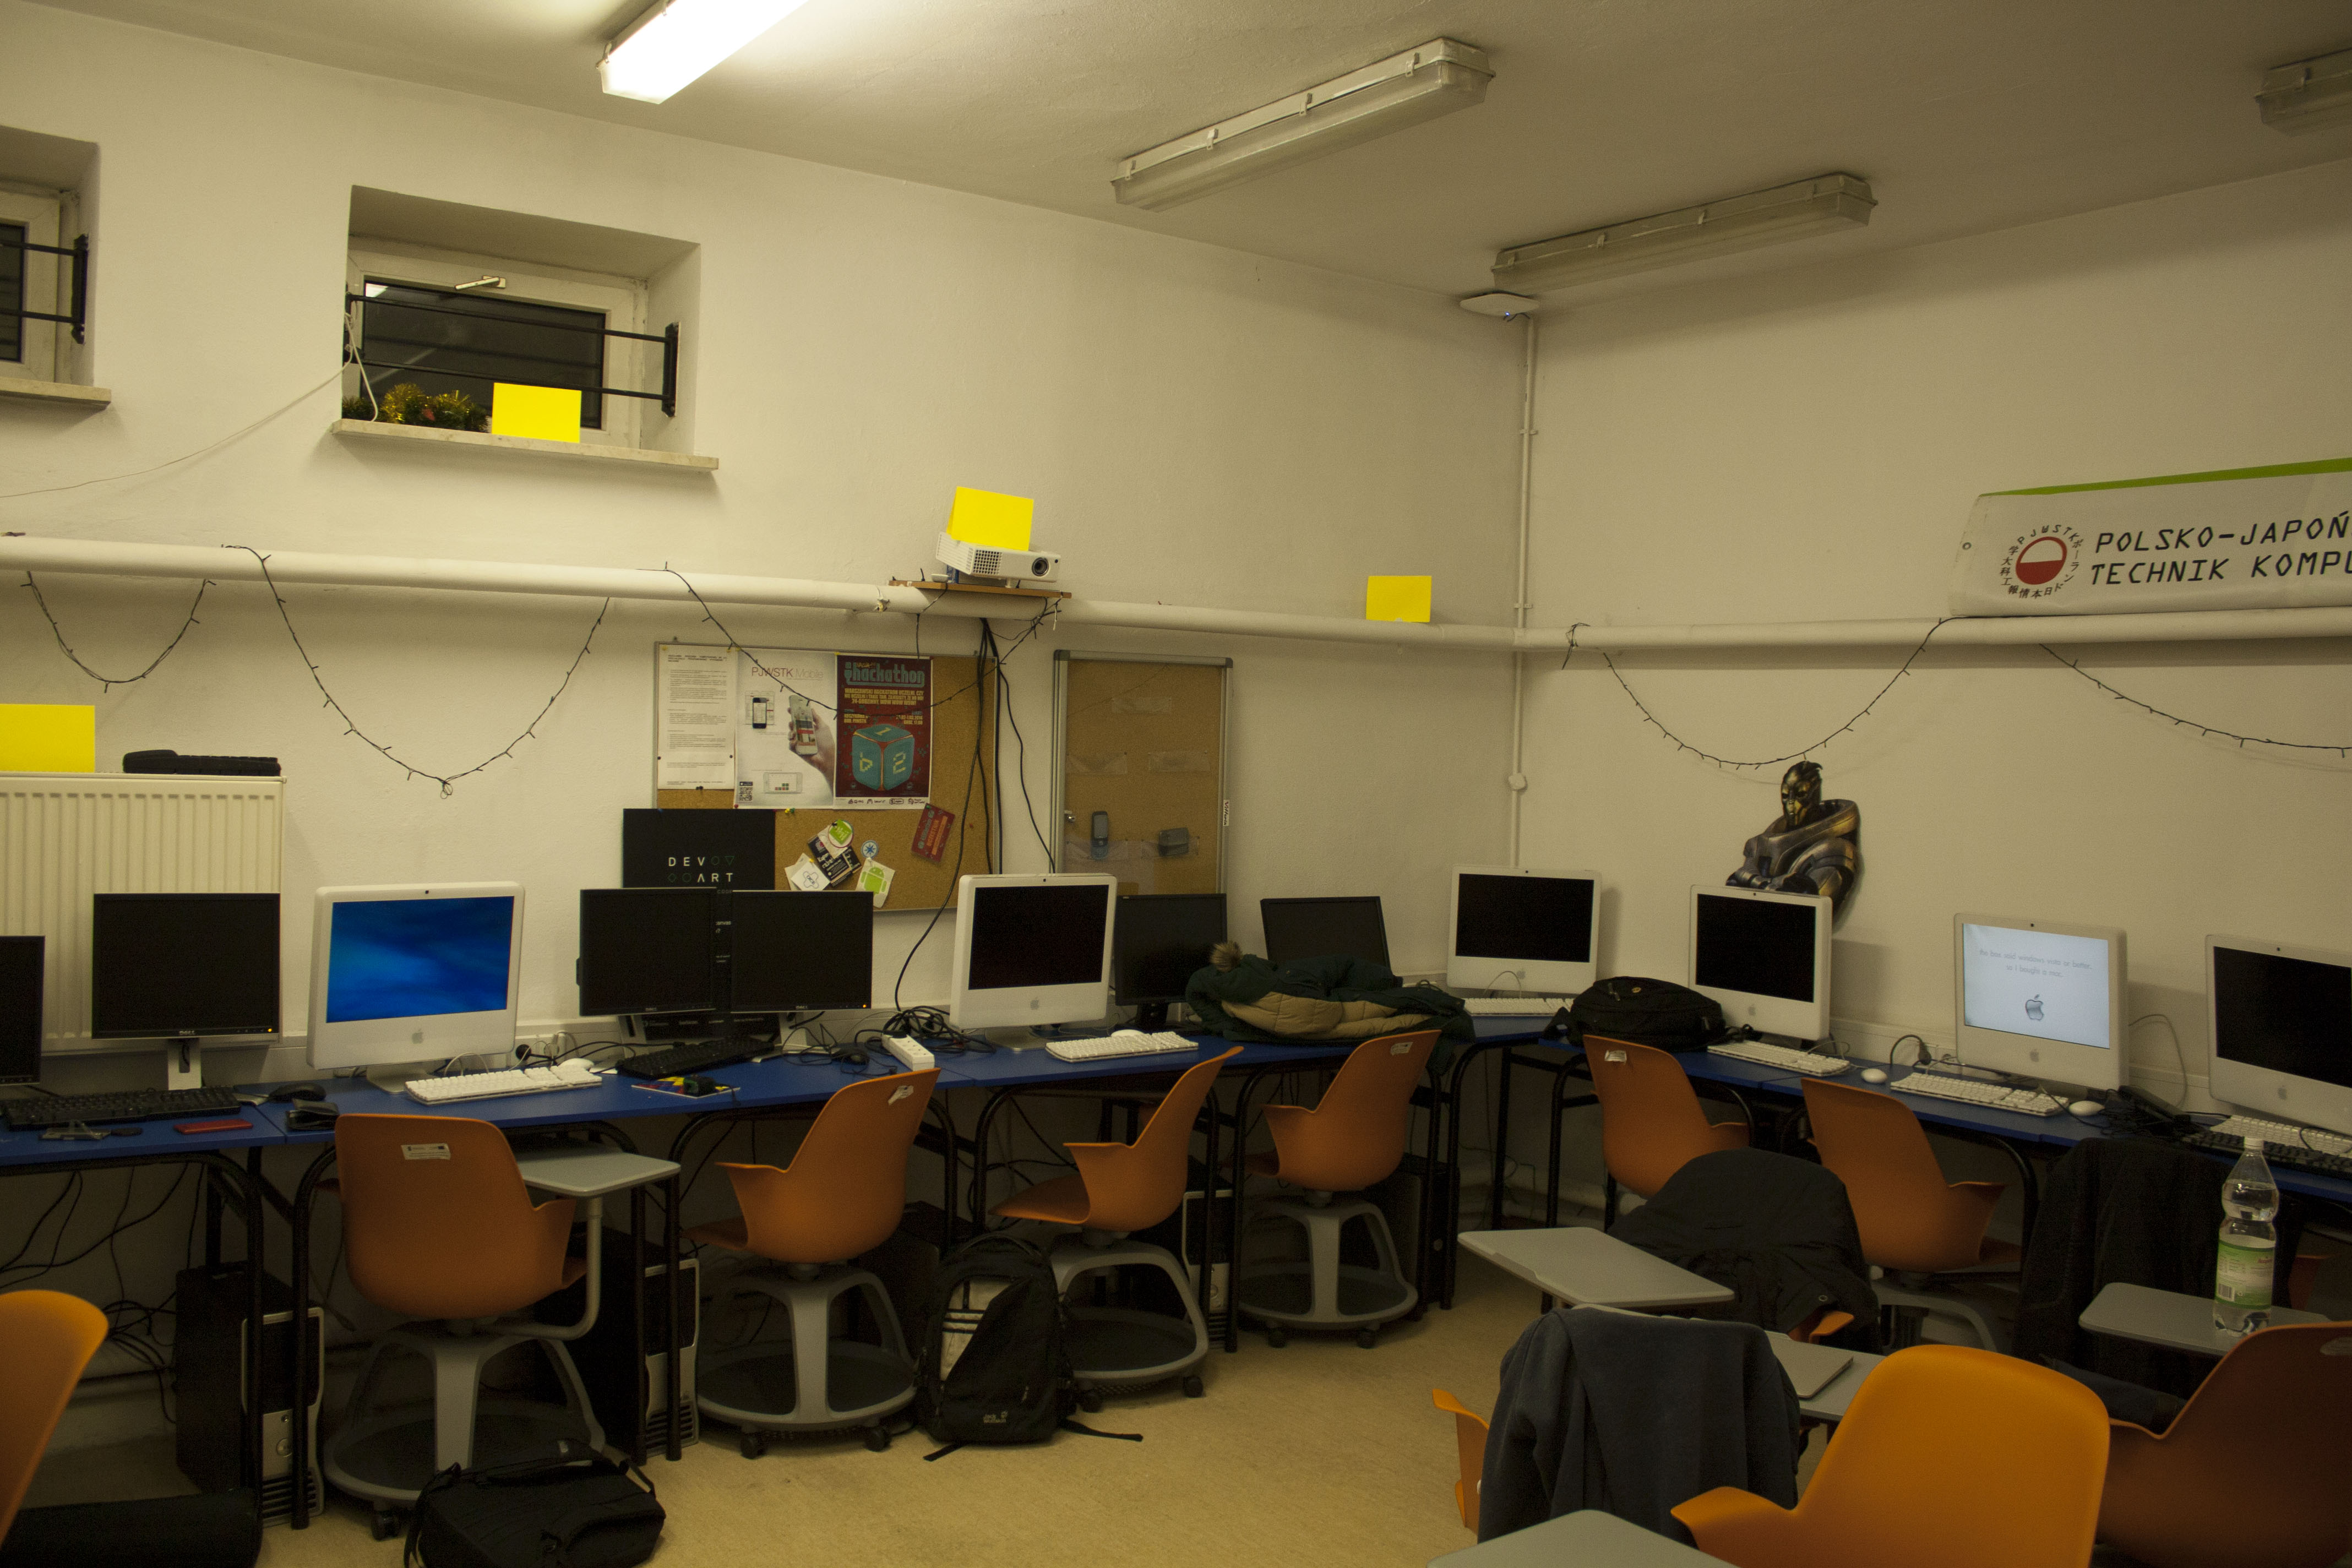
\includegraphics[width=0.9\textwidth]{images/s9.jpg}
\captionof{figure}{
Labolatorium PJATK
}
\small {źródło własne }
\end{center}

\paragraph{}
Głównym założeniem było stworzenie minigry opartej na grze z początku lat dziewiędziesiątych o nazwie Lemmingi \footnote{https://en.wikipedia.org/wiki/Lemmings}. Pierwotnie gra została stworzona w 1991 roku na platformę Amiga.

Celem gry jest doprowadzenie grupy aktorów (tytułowych Lemmingów) do wyjścia (mety). Aktorzy automatycznie idą w jedną stronę. Każdemu z nich można włączyć jedną lub więcej umiejętność (np. umiejętność kopania, swobodnego spadania - spadochron). Aktorzy generowani są automatycznie w określonej sekwencji czasu.

\subsection{Implementacja w technologii hologramu}
\paragraph{}
{\color{red}Tutaj opisać próby i przemyślenia na temat hologramu na drzwiach.}
\begin{center}
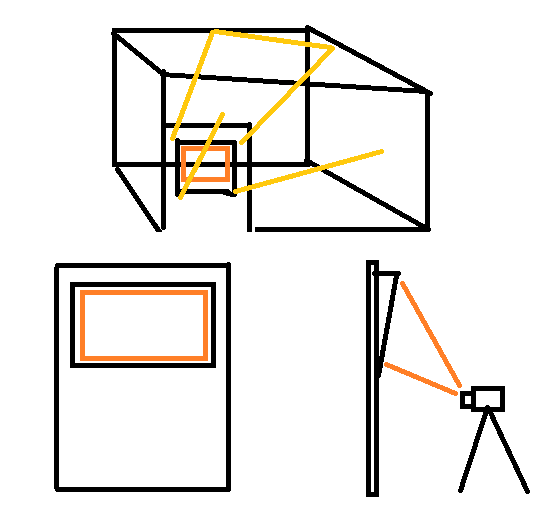
\includegraphics[width=0.9\textwidth]{images/hologramv1.png}
\captionof{figure}{
Poglądowy schemat działania
}
\small {źródło: własne }
\end{center}

\subsection{Implementacja w technologii mappingu 3d}
{\color{red}Tutaj opisać próby i przemyślenia + wstawić obrazek}